\begin{frame}
\frametitle{Key Points}
\begin{itemize}
\item We introduce the core concepts used in scheduling
\item Different layers of description
\begin{itemize}
\item What we are doing (jobs, tasks, resources)
\item Why we are scheduling (orders, products, processes)
\end{itemize}
\item Temporal Relations
\item Process description
\item Problem classification
\item Visualization
\end{itemize}
\end{frame}

\section{Core Concepts}


\subsection{Jobs, Tasks and Resources}

\begin{frame}
\frametitle{Most basic description of scheduling problem}
\begin{itemize}
\item \emph{Job}
\begin{itemize}
\item Collection of activities required to manufacture one object/lot/order
\item Overall start/end determined by starts and ends of its tasks
\end{itemize}
\item \emph{Task}
\begin{itemize}
\item Individual activities required for manufacture
\item Have defined start, end (typical: variables) and duration (sometimes fixed)
\item Often performed on one specific resource (more on that later)
\end{itemize}
\item \emph{Resources}
\begin{itemize}
\item Resources are needed to perform the tasks
\end{itemize}
\item Very compact representation of scheduling problem
\item But, where does that information come from?

\end{itemize}
\end{frame}

\subsection{Orders, Products, Processes}

\begin{frame}
\frametitle{Scheduling orders}
\begin{itemize}
\item An \emph{order} specifies a need for a certain \emph{product} at a given time in a specific quantity
\item There may be multiple ways of making the \emph{product} (multiple \emph{processes})
\item We assume that the process to use is decided when placing the order
\item Each order corresponds to a job, with its constituent tasks
\item There may be limited visibility of future orders
\end{itemize}
\end{frame}

\begin{frame}
\frametitle{Process Description}
\begin{itemize}
\item Each \emph{process} consists of one or more \emph{process steps}
\item A process step contains a duration formula to describe how long it lasts
\item The order of \emph{process steps} is defined by \emph{process sequences}
\item The resources needed are defined by \emph{resource needs} (described later on)
\item Tasks are created for each process step, their duration is based on the duration formula and order quantity
\end{itemize}
\end{frame}


\begin{frame}
\frametitle{Where do the orders come from?}
\begin{itemize}
\item Made to order
\begin{itemize}
\item Each order is caused by a customer request
\item Defines due date, release date often implied
\end{itemize}
\item Made to stock
\begin{itemize}
\item Orders are satisfied from stock
\item Inventory control strategy decides when to make product
\item Often called stock orders
\item More complex variant integrates production planning and detailed scheduling
\item Example later in course 
\end{itemize}
\end{itemize}
\end{frame}





\section{Temporal Relations}

\begin{frame}
\frametitle{Temporal Relations}
\begin{itemize}
\item Temporal constraints between tasks and/or jobs
\item Defined by the manufacturing process
\item In simple cases
\begin{itemize}
\item A single sequence of process steps performed in that order
\item Each task must finish before the next one can start
\end{itemize}
\end{itemize}

\includegraphics[width=\textwidth]{../02-concepts/images/sample-job}


\end{frame}



\subsection{Relations between Tasks}

\begin{frame}
\frametitle{The Most Common Relation: EndBeforeStart}
\begin{columns}
\begin{column}{0.5\textwidth}
\begin{itemize}
\item States that one task (T1) must end before the next one (T2) can start
\item Typical for manufacturing process based on the same item
\item Addition: offset
\begin{itemize}
\item Wait at least offset units between end and start
\item For example cooling, drying time outside a machine
\end{itemize}
\end{itemize}
\end{column}
\begin{column}{0.5\textwidth}
\scalebox{0.6}{
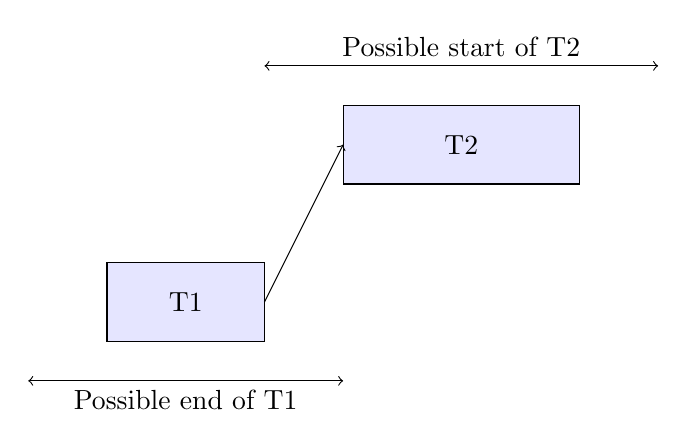
\begin{tikzpicture}
\draw[fill=blue!10,draw=black] (0,0) rectangle node {T1} (2,1);
\draw[fill=blue!10,draw=black] (3,2) rectangle node {T2} (6,3);
\draw[->] (2,0.5) -- (3,2.5);
\draw[<->] (2,3.5) -- node[above] {Possible start of T2}(7,3.5);
\draw[<->] (-1,-0.5) -- node[below] {Possible end of T1}(3,-0.5);
\end{tikzpicture}
}
\end{column}
\end{columns}
\end{frame}

\begin{frame}
\frametitle{Less Common: StartBeforeStart}
\begin{columns}
\begin{column}{0.5\textwidth}
\begin{itemize}
\item States that one task (T2) can start any time after the start of another task (T1)
\item Uncommon in manufacturing, occurs in project management
\item Example later on on assembly line balancing 
\end{itemize}
\end{column}
\begin{column}{0.5\textwidth}
\scalebox{0.6}{
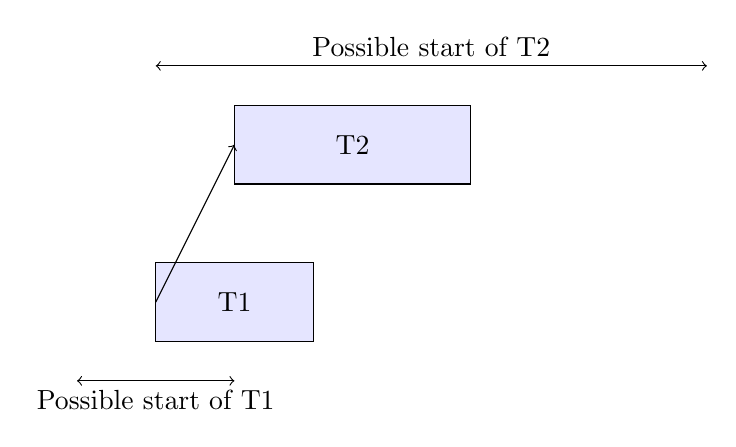
\begin{tikzpicture}
\draw[fill=blue!10,draw=black] (0,0) rectangle node {T1} (2,1);
\draw[fill=blue!10,draw=black] (1,2) rectangle node {T2} (4,3);
\draw[->] (0,0.5) -- (1,2.5);
\draw[<->] (0,3.5) -- node[above] {Possible start of T2}(7,3.5);
\draw[<->] (-1,-0.5) -- node[below] {Possible start of T1}(1,-0.5);
\end{tikzpicture}
}
\end{column}
\end{columns}
\end{frame}

\begin{frame}
\frametitle{NoWait}
\begin{columns}
\begin{column}{0.6\textwidth}
\begin{itemize}
\item Sometimes, two steps must follow each other immediately
\item The item made would spoil
\begin{itemize}
\item Product specific
\end{itemize}
\item There is no space to hold item
\begin{itemize}
\item Machine specific, buffers
\end{itemize}
\item End of one task (T1) must be equal to start of next task (T2)
\item May mean delay of start of task T1
\end{itemize}
\end{column}
\begin{column}{0.4\textwidth}
\input{../02-concepts/nowait}
\end{column}
\end{columns}
\end{frame}


\begin{frame}
\frametitle{MaxWait}
\begin{columns}
\begin{column}{0.6\textwidth}
\begin{itemize}
\item Limit how long we can wait between tasks
\begin{itemize}
\item Cooling enough, but not too much
\item Baking: rise time
\end{itemize}
\item Impose both lower and upper waiting time limit
\item Makes it more difficult to find solutions
\end{itemize}
\end{column}
\begin{column}{0.4\textwidth}
\input{../02-concepts/maxwait}
\end{column}
\end{columns}
\end{frame}

\begin{frame}
\frametitle{Blocking}
\begin{columns}
\begin{column}{0.5\textwidth}
\begin{itemize}
\item Sometimes, two steps must follow each other immediately
\item There is no space to store item between machines
\item Keep item on previous machine until needed
\item That machine is now \emph{blocked}
\item Duration of task T1 is extended until start of T2
\item \emph{Use with caution! Easy to deadlock}
\end{itemize}
\end{column}
\begin{column}{0.5\textwidth}
\scalebox{0.6}{
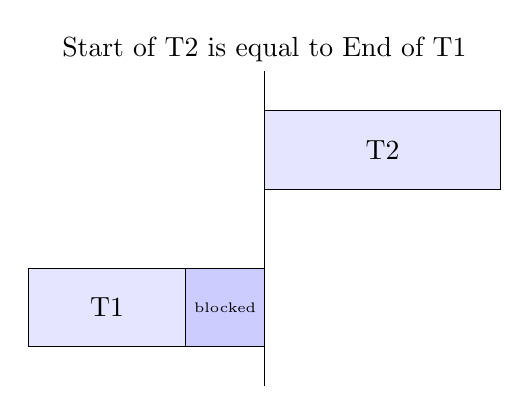
\begin{tikzpicture}
\draw[fill=blue!10,draw=black] (0,0) rectangle node {T1} (2,1);
\draw[fill=blue!20,draw=black] (2,0) rectangle node {\tiny blocked} (3,1);
\draw[fill=blue!10,draw=black] (3,2) rectangle node {T2} (6,3);
\draw[] (3,-0.5) -- (3,3.5) node[above] {Start of T2 is equal to End of T1};
\end{tikzpicture}
}
\end{column}
\end{columns}
\end{frame}

\begin{frame}
\frametitle{Special Case: Pipelining}
\begin{columns}
\begin{column}{0.5\textwidth}
\begin{itemize}
\item Sometimes, we can start on the next task while the first is still running
\item Possible if one jobs consists of multiple items (lots,...)
\item As soon as the first item is finished, take it to the next machine to process it there
\item Overlaps T1 and T2 as much as possible
\item Details can get complex
\end{itemize}
\end{column}
\begin{column}{0.5\textwidth}
\scalebox{0.6}{
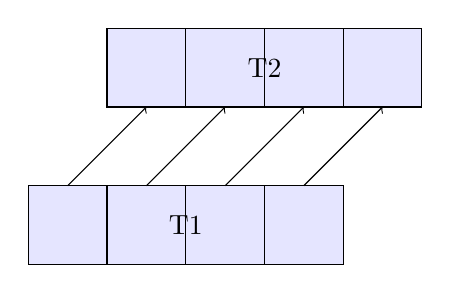
\begin{tikzpicture}
\draw[fill=blue!10,draw=black] (0,0) rectangle node {T1} (4,1);
\draw[fill=blue!10,draw=black] (1,2) rectangle node {T2} (5,3);
\draw (1,0) -- (1,1);
\draw (2,0) -- (2,1);
\draw (3,0) -- (3,1);
\draw (2,2) -- (2,3);
\draw (3,2) -- (3,3);
\draw (4,2) -- (4,3);
\draw[->] (0.5,1) -- (1.5,2);
\draw[->] (1.5,1) -- (2.5,2);
\draw[->] (2.5,1) -- (3.5,2);
\draw[->] (3.5,1) -- (4.5,2);
\end{tikzpicture}
}
\end{column}
\end{columns}
\end{frame}



\begin{frame}
\frametitle{More General: Relations between Intervals}
\begin{columns}
\begin{column}{0.5\textwidth}
\begin{itemize}
\item First introduced by Allen (1983)
\item 13 relations between intervals
\item Allows composition of relations
\item Constraint reasoning on sets of relations
\end{itemize}
\end{column}
\begin{column}{0.5\textwidth}
\includegraphics[width=\textwidth]{../02-concepts/images/allen-relations}

{\tiny from Wikipedia: \url{https://en.wikipedia.org/wiki/Allen\%27s_interval_algebra}}
\end{column}
\end{columns}
\end{frame}


\subsection{Relation between Tasks and Jobs}

\begin{frame}
\frametitle{Start and End of Jobs}
\begin{itemize}
\item The start of a job is equal to the start of the earliest task of the job
\item The end of a job is equal to the latest end of any of its tasks
\item Also called: the job \emph{spans} its tasks
\item Sometimes very simple
\begin{itemize}
\item Start of job is start of first process step
\item End of job is end of last process step
\item But, do we know which steps will be first or last?
\end{itemize}
\end{itemize}
\end{frame}

\begin{frame}
\frametitle{An Example of a Simple Process}
\includegraphics[width=\textwidth]{../02-concepts/images/simple-process}
\begin{itemize}
\item The steps form a precedence chain
\item Easy to identify first and last step
\end{itemize}

\end{frame}



\begin{frame}
\frametitle{An Example of a More Complex Process}
\includegraphics[width=\textwidth]{../02-concepts/images/complex-process}
\begin{itemize}
\item There is no clear first or last process step
\end{itemize}

\end{frame}



\subsection{Jobs: Release and Due Date}

\begin{frame}
\frametitle{Jobs: Release and Due Dates}
\begin{columns}
\begin{column}{0.5\textwidth}
\begin{itemize}
\item The execution of a job may be constrained in time
\item \emph{Release dates} states earliest time a job can start
\item \emph{Due dates} states latest time a job can end
\item These may or may not be hard constraints!
\item A job will be \emph{late} if it ends after the due date
\item A job will be \emph{early} if it ends before the due date
\item A job will be \emph{on-time} if it ends at the due date
\end{itemize}
\end{column}
\begin{column}{0.5\textwidth}
\scalebox{0.6}{
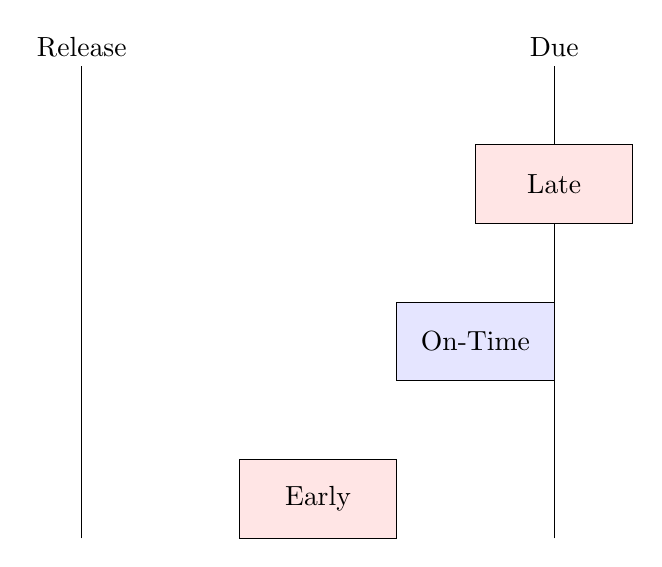
\begin{tikzpicture}
\draw (0,0) -- (0,6) node[above] {Release};
\draw (6,0) -- (6,6) node[above] {Due};
\draw[fill=red!10,draw=black] (2,0) rectangle node {Early} (4,1) ;
\draw[fill=blue!10,draw=black] (4,2) rectangle node {On-Time} (6,3) ;
\draw[fill=red!10,draw=black] (5,4) rectangle node {Late} (7,5) ;
\end{tikzpicture}
}

\end{column}
\end{columns}
\end{frame}


\subsection{Relations between jobs}

\begin{frame}
\frametitle{Relations between Jobs}
\begin{itemize}
\item There may be relations between jobs as well
\item For example, jobs for the same product may be arranged by due date
\item Do not allow to run job for a later due date before any job with an earlier due date
\item Orders for the same customer, but different products, may be constrained
\item Most common:
\begin{itemize}
\item Jobs for intermediate products must finish in time for their use later on
\end{itemize}
\end{itemize}
\end{frame}



\section{Alternative Processes, Bill of Materials}

\begin{frame}
\frametitle{More Complexity}
\begin{itemize}
\item We have ignored a lot of potential complications
\begin{itemize}
\item Alternative processes
\item Alternative process paths
\item Alternative resources
\end{itemize}
\item Intermediate products
\item Impact of raw material availability
\end{itemize}
\end{frame}

\begin{frame}
\frametitle{Intermediate products}
\begin{itemize}
\item Some production operations are assembly steps
\item Combine multiple intermediate products together
\item These intermediate products need to be made as well
\item There are processes for those products
\end{itemize}
\end{frame}

\begin{frame}
\frametitle{Raw materials}
\begin{itemize}
\item Sometimes, a process step needs certain raw materials 
\item These are not made within the scheduled part of the plant
\item They come from stock, inventory control problem
\item Do we schedule production and then order raw materials?
\item Do we schedule based on the available raw materials?
\end{itemize}
\end{frame}

\begin{frame}
\frametitle{Bill of Materials (BoM), Bill of Processes}
\begin{itemize}
\item Enterprise systems will describe which items are needed to make a product
\item Tree like structure, indicates the intermediate product/raw material needed and its quantity
\item \emph{BoM explosion} derive all required input materials for a given set of orders
\item We may want to know at which step of process we need which materials (Bill of processes)
\item This is where you use SAP, big database, trivial calculation
\item Becomes hard if processes not fixed
\end{itemize}
\end{frame}









\section{Problem Classification}

\begin{frame}
\frametitle{Problem Classification}
\begin{itemize}
\item Most real-world problems are messy, with many special conditions and exceptions
\item Academic research prefers well-structured problems
\item Scheduling research often focuses on well-structured problem types
\begin{itemize}
\item Easier to understand
\item Possible to exploit structure
\item Easier to compare results
\end{itemize}
\item A small number of problem types are very common in research
\end{itemize}
\end{frame}



\subsection{Job-Shop}

\begin{frame}
\frametitle{Job-Shop}
\begin{itemize}
\item Consists of a number of jobs and a number of machines
\item Each job visits each machine, but possibly in a different order, depending on process
\item Tasks of a job are linked as a precedence chain
\item Objective is to minimize overall end, the \emph{makespan}
\end{itemize}
\end{frame}

\begin{frame}
\frametitle{Example Job-Shop Process}
\includegraphics[width=\textwidth]{../02-concepts/images/job-shop-process}

\begin{itemize}
\item Note that the order of machines visited is different for each process
\end{itemize}
\end{frame}

\begin{frame}
\frametitle{Example Job-Shop Solution}
\includegraphics[width=\textwidth]{../02-concepts/images/job-shop-solution}

\begin{itemize}
\item One task is selected (in red), in both Machine and Job Gantt Chart
\end{itemize}
\end{frame}

\subsection{Flow-Shop}

\begin{frame}
\frametitle{Flow-Shop}
\begin{itemize}
\item Consists of a number of jobs and a number of machines
\item Each jobs visits each machine, all jobs in the same order
\item Tasks of a job a linked in a precedence chain
\item Objective is to minimize overall end, the \emph{makespan}
\end{itemize}
\end{frame}

\begin{frame}
\frametitle{}
\includegraphics[width=\textwidth]{../02-concepts/images/flow-shop-process}

\begin{itemize}
\item Note that each process visits the machines in order DR\_0, DR\_1, ...
\end{itemize}
\end{frame}

\begin{frame}
\frametitle{Example Flow-Shop Solution}
\includegraphics[width=\textwidth]{../02-concepts/images/flow-shop-solution}

\begin{itemize}
\item Tasks are colored by machine, note the regular pattern in the Job Gantt Chart
\end{itemize}
\end{frame}

\subsection{Open-Shop}

\begin{frame}
\frametitle{Open-Shop}
\begin{itemize}
\item Consists of a number of jobs and a number of machines
\item Each jobs visits each machine, we have to choose the sequence individually for each order
\item There are no temporal constraints between tasks, but tasks of the same job cannot overlap
\item Objective is to minimize overall end, the \emph{makespan}
\end{itemize}
\end{frame}


\begin{frame}
\frametitle{Open Shop Example Process}
\begin{columns}
\begin{column}{0.6\textwidth}
\begin{itemize}
\item Only showing details of one process
\item No prescribed sequence between process steps
\item Easier to find a task to run next
\item Much larger search space
\end{itemize}
\end{column}
\begin{column}{0.4\textwidth}
\includegraphics[width=.6\textwidth]{../02-concepts/images/open-shop-process}
\end{column}
\end{columns}
\end{frame}



\begin{frame}
\frametitle{Open-Shop Example Solution}
\includegraphics[width=\textwidth]{../02-concepts/images/open-shop-solution}

\begin{itemize}
\item Example solution for 7x7 open shop example
\item Order of tasks within jobs not constrained
\end{itemize}

\end{frame}




\subsection{RCPSP}

\begin{frame}
\frametitle{Resource Constrained Project Scheduling Problem (RCPSP)}
\begin{itemize}
\item Problem class from project management
\item One project (one job), many tasks
\item Precedence graph is arbitrary DAG
\item Cumulative as well as disjunctive resources
\item Variants with process alternatives
\end{itemize}
\end{frame}


\subsection{$\alpha/\beta/\gamma$ Notation}

\begin{frame}
\frametitle{$\alpha/\beta/\gamma$ Notation}
\begin{itemize}
\item The previous classes are good for research, but not very practical
\item General scheme to describe problem type introduced in 1979
\item Based on three parameters
\begin{description}
\item[$\alpha$] resource structure, stages
\item[$\beta$] temporal relations
\item[$\gamma$] objective
\end{description}
\item $P2/r_{j},\bar{d}_{j}/C_{\max}$ : One stage, two identical parallel machines, hard release and due dates, objective makespan
\item More detailed description at \url{https://encyclopedia.pub/entry/30497}

\end{itemize}
\end{frame}


\section{Key Visualization Methods}

\begin{frame}
\frametitle{Visualization}
\begin{itemize}
\item Visualization is key to present and to understand results
\item Many different ways to give an overview of schedule, and highlight problems
\item Some diagrams types are used a lot, and are provided in our generic scheduling tool
\item Customization is key
\end{itemize}
\end{frame}

\begin{frame}
\frametitle{Machine Gantt Chart}
\includegraphics[width=\textwidth]{../02-concepts/images/machine-gantt}

\begin{itemize}
\item Shows all tasks that are assigned to each machine
\item Tasks should not overlap
\item Also shows work in progress (WiP), down-times
\item Optional display of setup and idle times
\end{itemize}

\end{frame}

\begin{frame}
\frametitle{Job Gantt Chart}
\includegraphics[width=\textwidth]{../02-concepts/images/job-gantt}

\begin{itemize}
\item Shows all tasks of a job in one line
\item Only works for single chain of process steps
\item Possible display of earliness, lateness
\item Optional display of waiting and transport times
\end{itemize}

\end{frame}

\begin{frame}
\frametitle{Cumulative Resource Chart}
\includegraphics[width=\textwidth]{../02-concepts/images/cumulative-resource}

\begin{itemize}
\item Shows resource utilization of cumulative resource over time
\item Utilization should be below capacity profile
\item Unless we relax the cumulative resource constraint
\end{itemize}
\end{frame}

\begin{frame}
\frametitle{Cumulative Resource Constraint Relaxed}
\includegraphics[width=\textwidth]{../02-concepts/images/cumulative-relaxed}
\end{frame}



\begin{frame}
\frametitle{Resource Utilization}
\includegraphics[width=\textwidth]{../02-concepts/images/resource-utilization}

\begin{itemize}
\item Shows utilization of machines as percentage of active time
\item Helpful to identify bottleneck machines
\item Information also shown in Machine Gantt
\end{itemize}

\end{frame}

\begin{frame}
\frametitle{Intermediate Solutions}
\includegraphics[width=\textwidth]{../02-concepts/images/intermediate-solutions}

\begin{itemize}
\item Shows intermediate solutions found over time
\item Useful to see if enough/too much time is allocated
\end{itemize}

\end{frame}

\begin{frame}
\frametitle{Process Diagram}
\begin{columns}
\begin{column}{0.5\textwidth}
\begin{itemize}
\item See all details of one process in one image
\item Can also look at all processes in one diagram
\item Options to show/hide different fields
\end{itemize}
\end{column}
\begin{column}{0.5\textwidth}
\includegraphics[width=\textwidth]{../02-concepts/images/process-diagram}
\end{column}
\end{columns}
\end{frame}



\begin{frame}
\frametitle{PERT Chart(Program Evaluation Review Technique)}
\includegraphics[width=\textwidth]{../02-concepts/images/pert}

\begin{itemize}
\item Show details of job as a graph
\item Useful if task graph is not a chain
\item Often used in project management
\end{itemize}

\end{frame}

\begin{frame}
\frametitle{PERT Charts become Confusing Quite Quickly}
\includegraphics[width=\textwidth]{../02-concepts/images/pert-confusing}

\begin{itemize}
\item Especially if all resource dependencies are included (in blue)
\end{itemize}

\end{frame}






\section{Summary}

\begin{frame}
\frametitle{Summary}
\begin{itemize}
\item We introduced the key concepts for scheduling problems
\item Orders, products, processes
\item Jobs and tasks
\item Existing problem classifications
\begin{itemize}
\item Academic
\item Limited practical usefulness
\item Used for benchmarking
\end{itemize}
\item Key visualization ideas
\end{itemize}
\end{frame}

